\section{Experiments}

We have implemented and trained our SAMNet model using MI-Prometheus~\cite{kornuta2018accelerating}, a framework based on Pytorch~\cite{paszke2017automatic}.
We evaluated the model on the COG dataset~\cite{yang2018dataset}, a video reasoning~\cite{mogadala2019trends} dataset developed for the purpose of research on relational and temporal reasoning. We have also evaluated the model's performance on the CLEVR dataset~\cite{johnson2017clevr}, created for Image Question Answering research.
Our experiments were designed to study SAMNet's performance as well as its generalization abilities in different settings.
For this purpose, we used two variants of the COG dataset: an easy one (Canonical) and a Hard version. The main differences are the number of frames in the input sequence (4 vs. 8) and the maximum number of distractors (i.e., objects not relevant for the answer) per single frame (1 vs. 10).
For CLEVR, we considered the CoGenT (Constrained Generalization Test) variant which contains two conditions, differing on the combinations of attributes values. More details on the composition of these datasets is available in Appendix \ref{sec:datasets-desc}.

\subsection{Performance comparison with the COG baseline}

In our experiments, we have trained SAMNet using 8 reasoning steps and the external memory having 8 address locations, each being a vector of 128 floats.
%We have also carried out experiments with different numbers of reasoning steps and memory size, but this goes beyond the scope of this paper.
We focused on 22 classification tasks and compared our results with the baseline model.
The most important results are highlighted in~\cref{fig:samnet_cog_detailed}, whereas full comparison can be found in Appendix~\ref{sec:cog-all-results}.

\begin{figure*}[htb]
	\centering
	\begin{subfigure}{\textwidth}
		\centering
		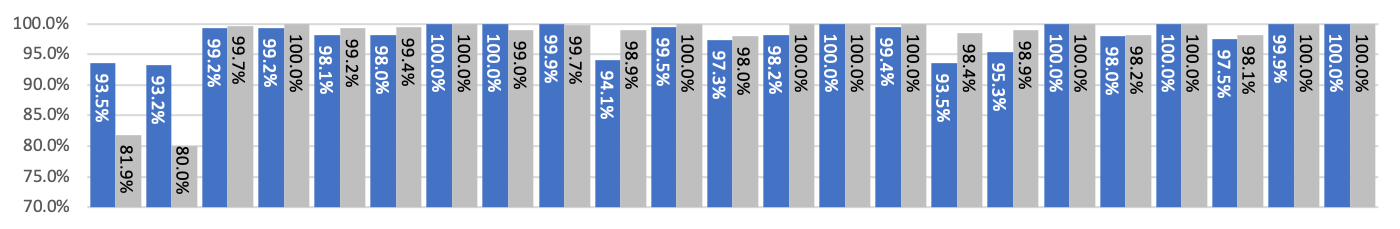
\includegraphics[width=0.9\textwidth]{img/results/samnet_cog_orig_canonical_no_labels.png}
	\end{subfigure}%
	\newline
	\begin{subfigure}{\textwidth}
		\centering
		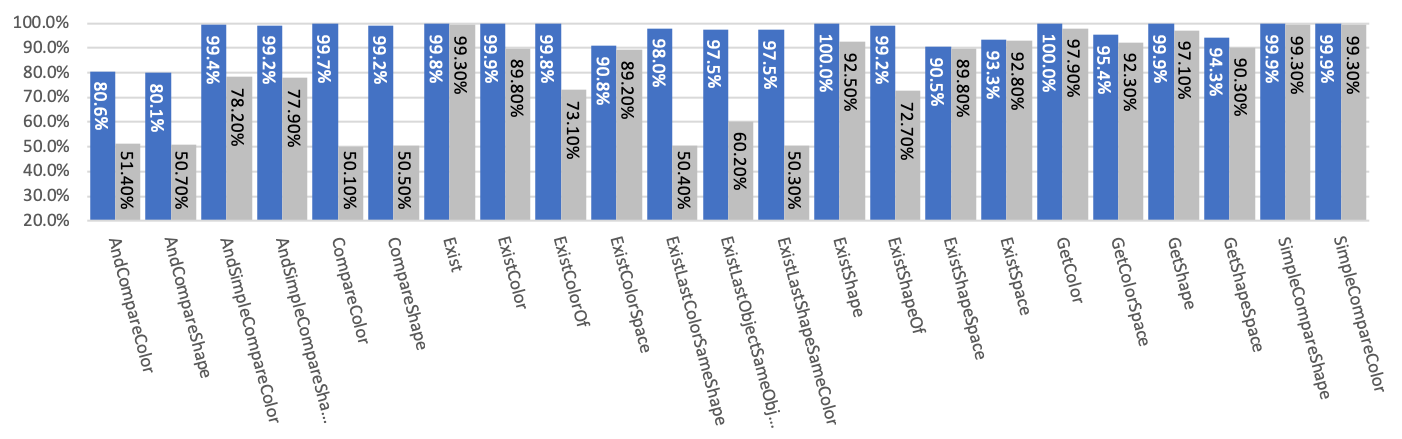
\includegraphics[width=0.9\textwidth]{img/results/samnet_cog_orig_hard.png}
	\end{subfigure}%
	\caption{Comparison of test set accuracies of SAMNet (blue) with original results achieved by the COG model (gray) on Canonical (top) and Hard (bottom) variants of the COG dataset.}
	\label{fig:samnet_cog_detailed}
\end{figure*}

For the Canonical variant (top row), we have achieved similar accuracies for the majority of tasks (with the total average accuracy of 98.0\% in comparison of 97.6\% achieved by the COG model), with significant improvements (around 13 points) for \textit{AndCompare} tasks.
As those tasks focus on compositional questions referring to two objects, we hypothesize that our model achieved better accuracy due to the ability to selectively pick and store the relevant objects from the past frames in the memory.
Despite there being some tasks in which our model reached slightly lower accuracies,
% (between 0.2 and 1.8 points)
when comparing performances on the Hard variant, it improves upon the COG baseline on all tasks, with improvements varying from 0.5 to more than 30 points.

\subsection{Temporal generalization capabilities}

The goal of the next set of experiments was to test the generalization ability concerning the sequence length and number of distractors.
For that purpose, we have compared the accuracies of both models when trained on the Canonical variant and tested on Hard (\cref{fig:samnet_cog_overall_transfer}).
As the original paper does not include such experiments, we have performed them on our own. The light gray color indicates the original results, whereas dark gray indicates the accuracies of COG models that we have trained (fine-tuning/testing) using the original code provided by the authors.
For sanity check, in the first column, we report both the best-achieved score and the score reported in the paper when training and testing on Canonical variant, without any fine-tuning.
In a pure \textit{zero-shot learning} setup (second column), our model shows enormous generalization ability, reaching 91.6\% accuracy on the test set.
We have also tested both models in a setup where the model trained on a Canonical variant underwent additional fine-tuning (for a single epoch) on the Hard variant (third column).
In this case, the SAMNet model also reached much better performance, and, interestingly, achieved better scores from the model trained and tested exclusively on the Hard variant.

\begin{figure}[htb]
	\centering
	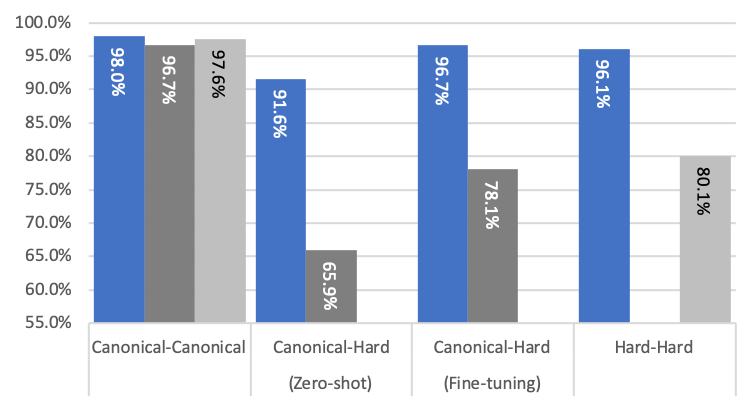
\includegraphics[width=0.5\textwidth]{img/results/samnet_cog_overall_transfer.png}
	\caption{Total accuracies of SAMNet (blue) and COG models (light/dark gray) when testing generalization from Canonical to Hard variants of the dataset.}
	\label{fig:samnet_cog_overall_transfer}
\end{figure}

\subsection{Multi-task learning on CLEVR and COG tasks}

%We have trained SAMNet using MI-Prometheus~\cite{kornuta2018accelerating}, a framework based on PyTorch~\cite{paszke2017automatic}, using the training set of the condition A of the CLEVR dataset (CLEVR-CoGenT)~\cite{johnson2017clevr}.
%For all experiments, the training procedure is as follows: we train the model for 20 epochs on 90\% of the training set of CoGenT. We keep the remaining 10\% for validating the model at every epoch, and use the original validation sets (CoGenT-A  \& -B) as test sets. We used NVIDIA's GeForce GTX TITAN X GPUs.

For the CLEVR dataset, we consider as task groups the question categories defined by the authors: \textit{Exist}, \textit{Count}, \textit{CompareInteger}, \textit{CompareAttribute}, \textit{QueryAttribute}. In order to investigate the potential benefits of multi-task learning, we conducted the following experiments:

\begin{itemize}
	\compresslist
	\item We first trained SAMNet on a single task group $t$, and tested on this same task group. These 5 experiments fit into the traditional Deep Learning procedure of single-task learning.
	\item Following, we trained SAMNet on all task groups jointly, and evaluated its performance on each task $t$ separately.
	\item Finally, for each task group $t$, we trained SAMNet on all tasks but $t$, and tested its performance on $t$. These experiments steer away from single / multi-task training and rather fall under the Domain Adaptation setting, categorized as \emph{transductive} transfer learning in \cite{pan2009survey}.
\end{itemize}

\begin{figure}[!t]
	\centering
	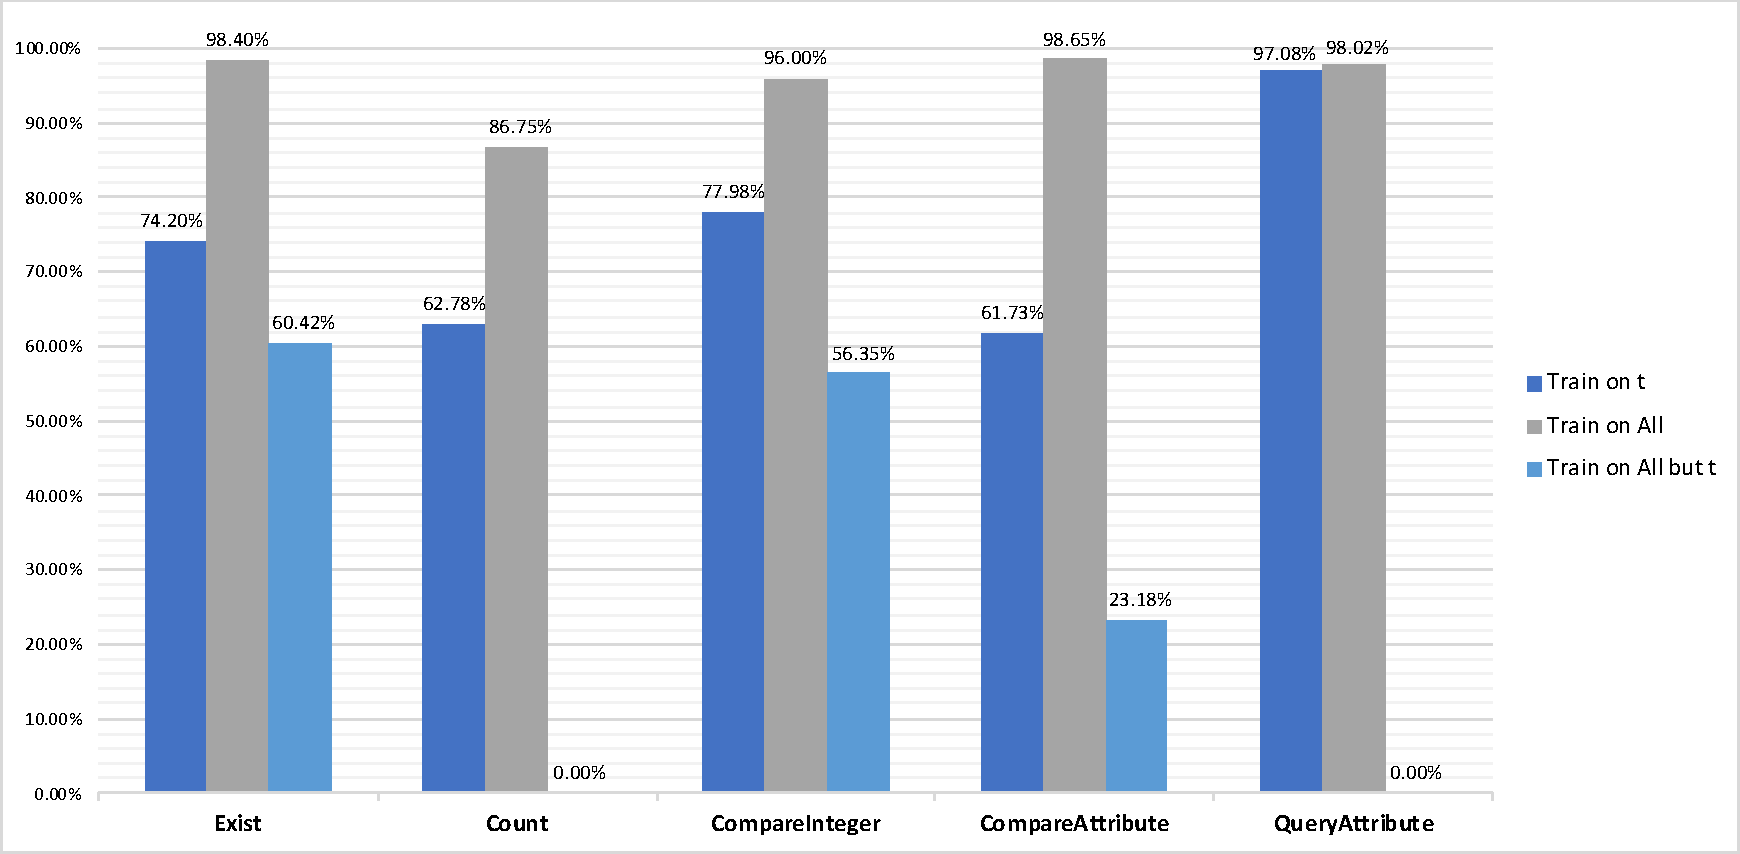
\includegraphics[width=0.5\textwidth]{img/results/CoGenT_results.pdf}
	\caption{CLEVR-CoGenT accuracies for all tasks $t$ when training on $t$ only, training on all tasks jointly and training on all tasks but $t$. For all experiments, the validation and test sets are identical.}
	\label{fig:CoGenT-results}
\end{figure}

The results of these experiments are available in \Fig{fig:CoGenT-results}. The complete set of results is available in Appendix \ref{sec:full-cogent-results}.


Looking at \Fig{fig:CoGenT-results}, we observe that single-task learning results in better-than-average performance on the same task. \textit{Exist}, \textit{CompareInteger} and \textit{CompareInteger} are binary tasks; \textit{Count} has for corresponding labels the digits 0 through 10 (a random agent would thus obtain $\sim$9.1\% accuracy) and \textit{QueryAttribute} maps to the set of object attributes values (15 labels). In that perspective, SAMNet does well on \textit{Count} and \textit{QueryAttribute}, but poorer on the 3 other tasks.

Nonetheless, significant accuracy gains are observed when training jointly on all 5 tasks. We indeed observe improvements ranging from 18 points to 37 points on 4 out of 5 tasks. \textit{QueryAttribute} does not benefit from such an improvement, only seeing an increase of one point. One could qualify it as \textit{self-sufficient}, as single- and multi-task learning performance are close.
These accuracy improvements thus suggest that related tasks benefit from joint training. % i.e. \emph{the whole is greater than the sum of the parts}.
To increase the granularity of the observed improvements, we plan to run additional experiments to jointly train on $t$ and all possible subsets of the remaining 4 tasks. We hypothesize that the improvements on e.g. \textit{Exist} would mostly originate from training jointly on \textit{CompareAttribute} and \textit{CompareInteger} since all 3 tasks share the same output space (i.e. labels domain).
% 5 x 2^4 = 80 experiments to get that granularity.

Finally, the "all-tasks-but-$t$" experiments demonstrate that while task groups are related, one does not subsume another in terms of learning. Indeed, we can observe that for \textit{CompareAttribute}, while \textit{Exist} and \textit{CompareInteger} share the same output space, including them and holding out \textit{CompareAttribute} from the training set results in poor accuracy. We also observe accuracy of zero for \textit{Count} and \textit{QueryAttribute}. This is due to these tasks having distinct labels domains, which do not overlap with the other tasks. Thus, if holding out samples from \textit{Count} during training, a model will not be able to learn to predict the corresponding labels.

 
A final set of experiment, for which the results are available in Appendix \ref{sec:full-cogent-results}, finetuned the model trained on all tasks on each task $t$ respectively. Given the initial training on all tasks, we were interested in the tradeoff between the performance gain, if any, on the finetuned task and the drop, if any, on the other tasks. Finetuning did not demonstrate a statistically meaningful benefit (except for \textit{Count}, where the accuracy increased by 1.5 pt) without hurting performance on the other tasks. Nevertheless, these experiments leave open the possibility that the training method for multi-task training could potentially benefit from using weighted sampling towards the tail end with more emphasis on samples from less performing task groups. Recent work~\cite{guo2018dynamic, kendall2018multi} in this direction has been done, although seems to weigh the tasks rather than samples.

\subsection{Domain Adaptation}

\vm{todo...}